\documentclass[a4paper,10pt]{article}
\usepackage[utf8]{inputenc}
\usepackage{graphicx}
\usepackage{float}
\usepackage{amsmath}
\usepackage{amssymb}
%opening
\title{}
\author{Zack Garza}

\begin{document}

\section{Examples of Trees}
\begin{figure}[H]
	\begin{centering}
	\begin{center}
	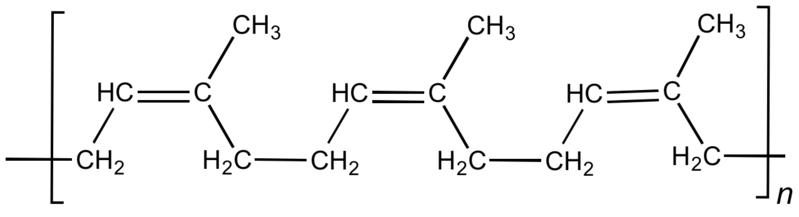
\includegraphics[width=\linewidth]{./Pictures/chemistry.png}
	\caption{Cis-polyisoprene, the main constituent of natural rubber, and many other hyrdocarbons can be represented as connected graphs, and thus trees as well. Nonisomorphic trees with the same number of vertices correspond to isomers.}
	\label{fig:chem}
	\end{center}
	\par\end{centering}
\end{figure}

\begin{figure}[H]
	\begin{centering}
	\begin{center}
	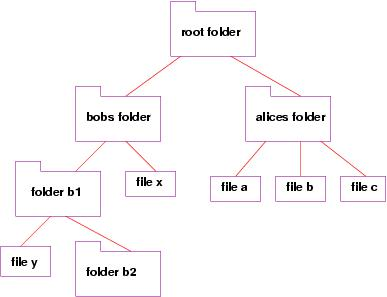
\includegraphics[width=\textwidth]{./Pictures/tree.png}
	\caption{Tree representation of a directory structure, corresponding to an undirected graph.}
	\label{fig:directory}
	\end{center}
	\par\end{centering}
\end{figure}

\begin{figure}[H]
	\begin{centering}
	\begin{center}
	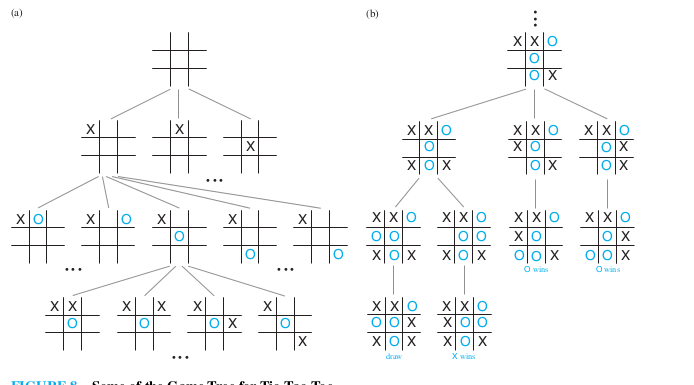
\includegraphics[width=\linewidth]{./Pictures/game_states.png}
	\caption{Portion of a game state tree from Tic-Tac-Toe}
	\label{fig:game_state}
	\end{center}
	\par\end{centering}
\end{figure}

\begin{figure}[H]
	\begin{centering}
	\begin{center}
	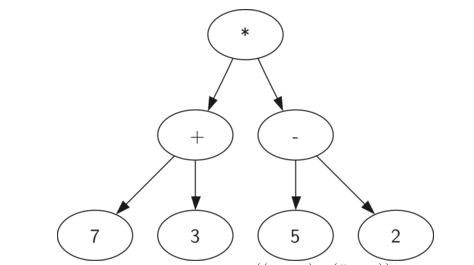
\includegraphics[width=\linewidth]{./Pictures/parse_tree.png}
	\caption{A tree that parses mathematical operators, preserving their ordering.}
	\label{fig:parse}
	\end{center}
	\par\end{centering}
\end{figure}

\begin{figure}[H]
	\begin{centering}
	\begin{center}
	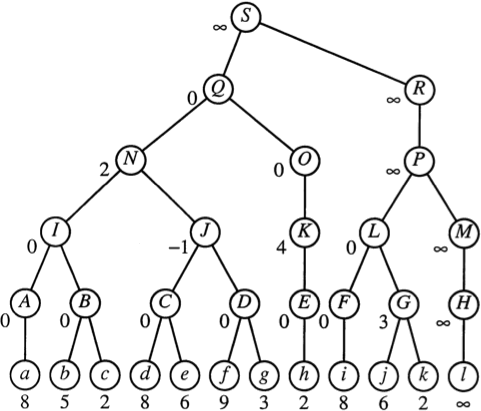
\includegraphics[width=\linewidth]{./Pictures/topology-tree.png}
	\caption{Tree with weighted edges, again undirected.}
	\label{fig:toplogy}
	\end{center}
	\par\end{centering}
\end{figure}

\section{Rooted Trees}

\begin{figure}[h!]
	\begin{centering}
	\begin{center}
	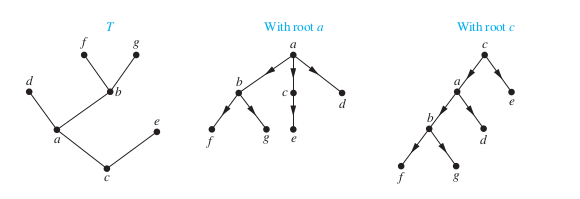
\includegraphics[width=\linewidth]{./Pictures/changing_roots.png}
	\caption{Changing the root of $T$ from $a$ to $c$. Notice that the direction between $a$ and $c$ is reversed when the roots are changed.}
	\label{fig:changing_roots}
	\end{center}
	\par\end{centering}
\end{figure}

\end{document}
